\begin{theo}[Demand function]{Demand function and the inverse demand function}
    \begin{itemize}
        \item 
            The demand function $x_D(p)$ illustrates the demand for a certain good at a certain price, see the following illustration:
            \begin{center}
                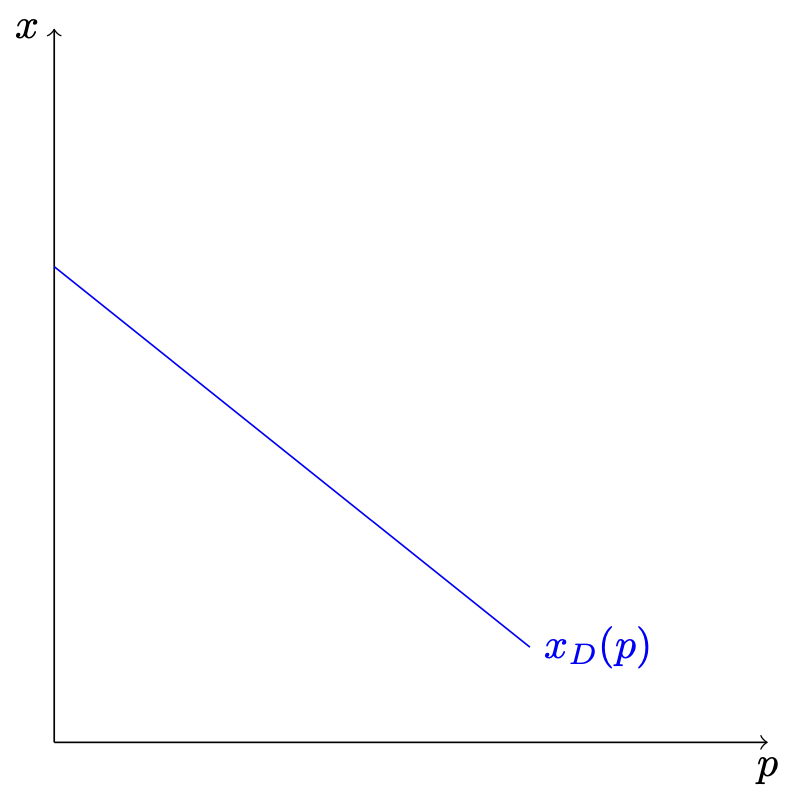
\includegraphics[scale = 0.2]{Images/Demand/DemandFunction.png}
            \end{center}
            The demand function is decreasing: $p \uparrow \ \Rightarrow x_D(p) \downarrow$
        \item  
            The inverse demand function $v(x)$ illustrates the consumers willingness to pay for a good, see the following illustration:
            \begin{center}
                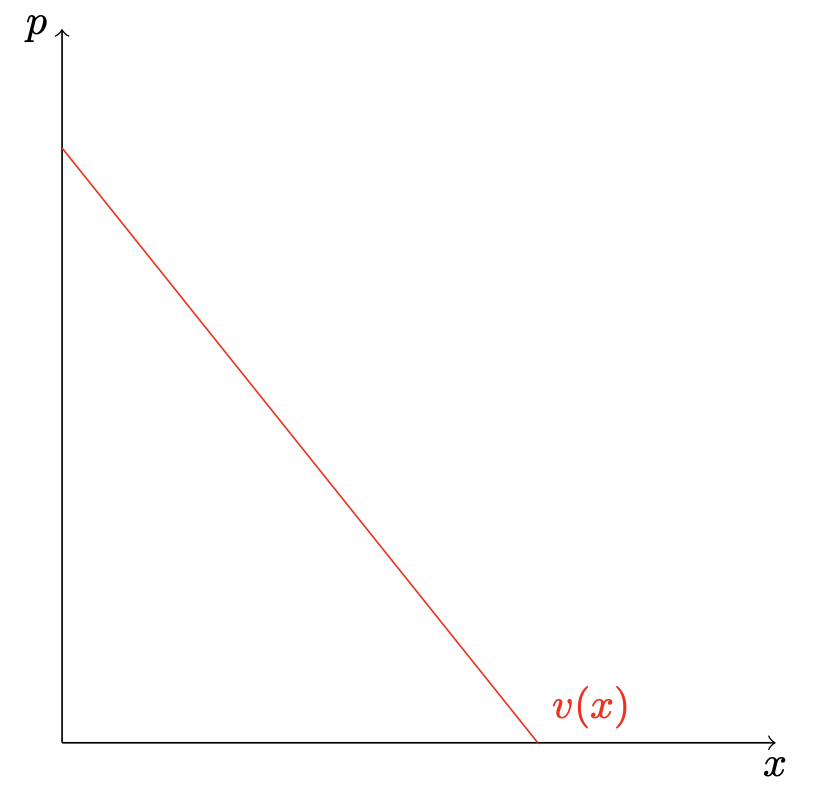
\includegraphics[scale = 0.2]{Images/Demand/InverseDemandFunction.png}
            \end{center}
            An agent will be willing to buy more as long as $v(x) > p$. 
    \end{itemize}
\end{theo}

\newpage

\begin{theo}[Utility function]{Utility function}
    The utility function illustrates the total monetary value of total consumption:
    \begin{equation*}
        u(x) = \int_0^x v(s)ds
    \end{equation*} 
    We can also refer to $v(x)$ as the agent's \textbf{marginal utility function}, since 
    \begin{equation*}
        u'(x) = v(x).
    \end{equation*}
    Since we required $v(x)$ to be decreasing in $x$, this means that $u(x)$ is concave:
    \begin{equation*}
        u''(x) = v'(x) < 0.
    \end{equation*}
    \vspace*{-0.5cm}
\end{theo}

\begin{theo}[Cosumer surplus]{Cosumer surplus}
    The consumer surplus $CS$ is the consumer's utility net of the monetary cost of consumption:
    \begin{equation*}
        CS = u(x) - px = \int_0^x v(s)ds - \int_0^x pds = \int_0^x \left(v(s) - p \right)ds
    \end{equation*}
    Graphically, the consumer surplus is definedned as the area that lies below the inverse demand function, but above the price line:
    \begin{center}
        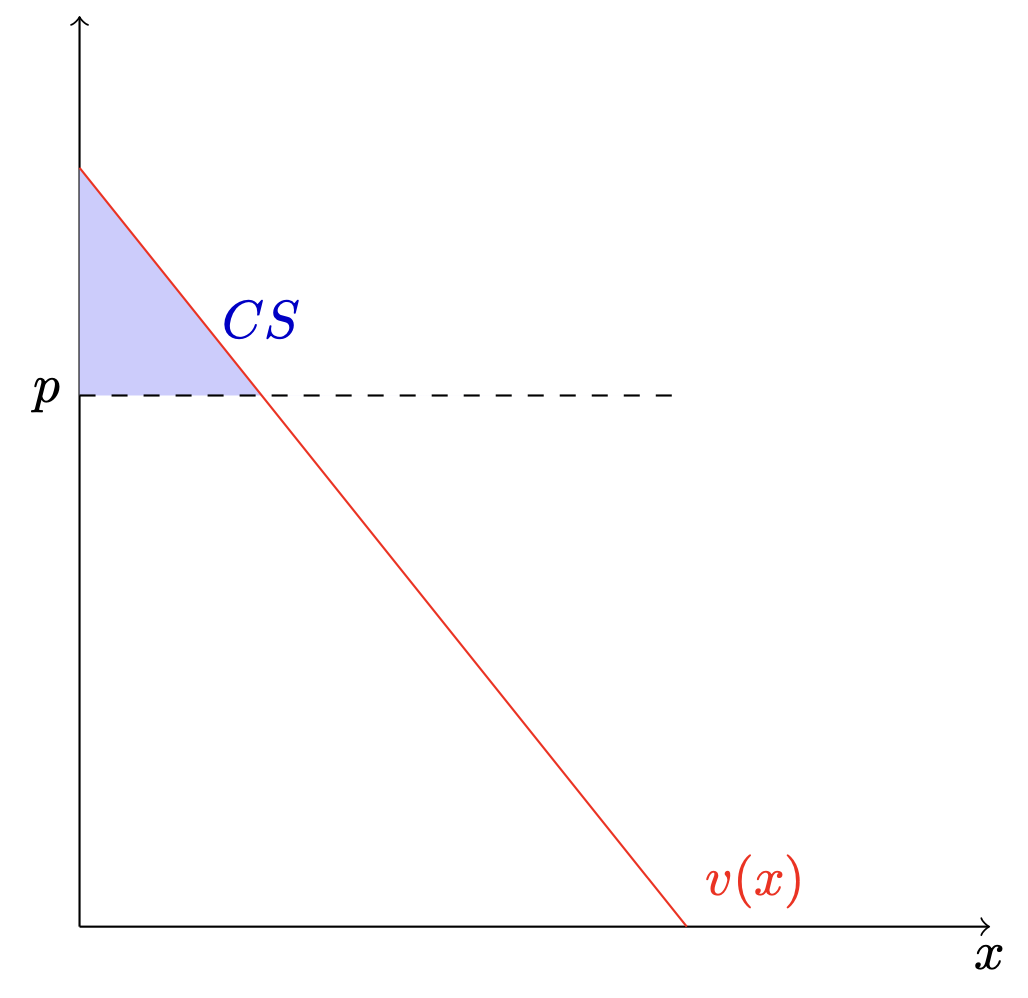
\includegraphics[scale = 0.15]{Images/Demand/ConsumerSurplus.png}
    \end{center}
    When deciding to buy a good, an agent is maximizing consumer surplus, i.e., the net benefit of consumption:
    \begin{equation*}
        \max_x \ CS = \max_x \ u(x) - px
    \end{equation*}
\end{theo}